\documentclass[10pt,a4paper]{article}
\usepackage[utf8]{inputenc}
\usepackage[spanish, es-tabla]{babel}
\usepackage{listings}
\usepackage{pdfpages}
\usepackage{pythontex} 
\usepackage{amsmath}
	\numberwithin{equation}{section}
	\numberwithin{figure}{section}
	\numberwithin{table}{section}
\usepackage{subfigure}
\usepackage{booktabs}
\usepackage[hang,bf,justification=centering]{caption}
\usepackage{amsfonts}
\usepackage{amssymb}
\usepackage{gensymb}
\usepackage{lscape}
\usepackage{gensymb}
\usepackage{hyperref}
\usepackage[normalem]{ulem}
\useunder{\uline}{\ul}{}
\usepackage{algorithm,algorithmic}

\usepackage{graphicx}
	\graphicspath
	{
		{Images/} 
	}
\usepackage{indentfirst}
\usepackage{geometry}
 	\geometry
 	{
		a4paper, 
		total	= {210mm,297mm},
		left	= 20mm,
		right	= 20mm,
		top		= 20mm,
		bottom	= 20mm,
	}
\usepackage{float}
\usepackage{fancyhdr}
\pagestyle{fancy}
\rhead{Dr. Rodriguez, Daniel -  Manchiunas, Valeria}
\lhead{75.12 - Análisis Numérico}
\lfoot{Moreno,Vicari}
\rfoot{Universidad de Buenos Aires}
\cfoot{\thepage}

\begin{document}

% ----------------------%
% 		CARATULA 		%
%-----------------------%

\title{TP 1 NUMÉRICO }    


\begin{titlepage}
%%%%%%%%%%%%%%%%%%%%%%%%%%%
%%%%%%%%%%%%%%%%%%%%%%%%%%%%%%%%%555
	\vspace*{30mm}

	\begin{center}
	    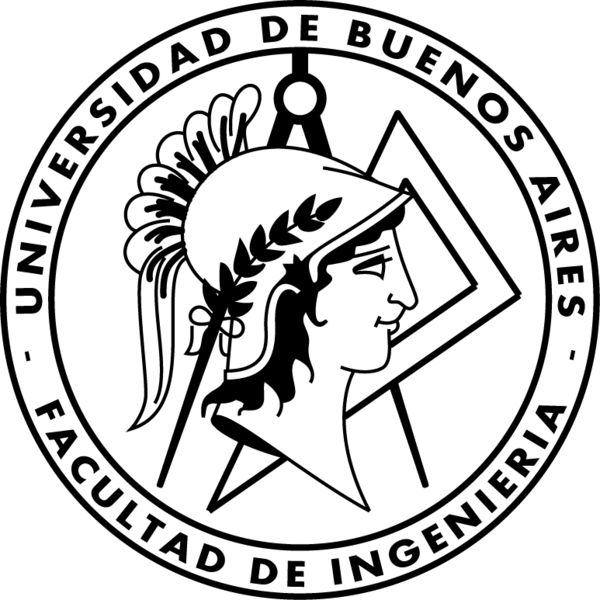
\includegraphics[scale=1.2]{../Images/Logo_Fiuba2.png}\\
		\huge{\textsc{Universidad de Buenos Aires}}\\
		\huge{\textsc{Facultad de Ingeniería}}\\
		\vspace*{5mm}
		\large{Año 2021 - 1.\textsuperscript{er} cuatrimestre}
	\end{center}

	\vspace*{15mm}

	\begin{center}
		\huge{\underline{\textsc{ANÁLISIS Y NUMÉRICO (75.12 - 95.04)}}}\\
		\vspace*{5mm}
		\large{Curso 06 - Rodriguez - Machiunas}
	\end{center}

	\vspace*{5mm}

	\begin{large}
			
	\begin{tabbing}
		\hspace{15mm} \= \+	
		\textsc{TRABAJO PRÁCTICO DE MÁQUINA N.º 1}\\
		
         
		\textsc{Integrantes:}\\
	
%	\vspace*{10mm}
	
		\begin{tabular}{ l l l }
			
          
			
            
             86559 & Vicari, Dario Santiago		&  dvicari@fi.uba.ar\\
             88019 & Moreno, Jorge              &  jomoreno@fi.uba.ar\\
             

		\end{tabular}
	 
	\end{tabbing}
	
	\end{large}
	
	\hspace{15mm} \textsc{Fecha de entrega:} 12/06/2021  	\hspace{15mm} 
	
\end{titlepage}


\setcounter{page}{1}


\section{\underline{Enunciado}}

La altura de las mareas se puede modelar utilizando una sumatoria de componentes armónicas de acuerdo a la siguiente ecuación:

\begin{equation}\label{eq_1}
\begin{split}
altura = a_0 + \Big[\sum_{k=1}^{n} a_k  \cos(\omega_k t + \Phi_k)\Big] 
\end{split}
\end{equation}


siendo:\\
$a_0$: nivel medio de referencia\\
$n$: número de componentes armónicas consideradas\\
$\omega_k$: frecuencia angular de la componente armónica k-ésima\\
$\phi_k$: fase de la componente armónica k-ésima\\

Los parámetros de la ecuación \ref*{eq_1} se calculan a partir de la serie temporal de datos obtenida por mareógrafos en los años anteriores, conocida como marea astronómica. Por lo general los responsables de la toma de datos de los mareógrafos son organismos que dependen de los gobiernos.\\
Históricamente se realizaba una publicación llamada anuario de mareas y en ocasiones también se publicaban las últimas constantes armónicas obtenidas en los puertos principales.\\
Actualmente parte de la información es de acceso público a través de páginas web. Por ejemplo, en Argentina, el organismo responsable es el Servicio de Hidrografía Naval. \url{http://www.hidro.gov.ar}. Cada puerto tiene asociada una tabla de mareas y en ocasiones hay que realizar correcciones debido a la influencia de los factores meteorológicos.\\
\\
El primer objetivo de este TP es estimar las constantes armónicas de un puerto, del cual se dispone la altura de la marea en forma horaria, durante un año.\\
\\
Cada grupo elegirá una combinación de puerto/año diferente, de un conjunto suministrado por los docentes.[ Publique en el foro del TP 1 su puerto/año de esta primer parte, y verifique que no haya sido elegido por otro grupo]\\
\\
Para cumplir adecuadamente el objetivo propuesto se sugiere se realicen los siguientes pasos:
\begin{enumerate}
    \item 
    Determinen las frecuencias angulares más importantes $(\omega_1$,$\omega_2$,$\omega_3$,...$\omega_n)$. Para ello utilicen la transformada discreta de Fourier. Podrán utilizar la implementación de la transformada rápida de Fourier (fft) en Octave o Python. Deberán indicar que criterio utilizan para definir la cantidad de componentes armónicas ($n$). (En caso de consultar bibliografía adicional, recuerden tomar nota de los datos de la misma, para citarla en la bibliografía).
    \item
    Utilicen el método de mínimos cuadrados para obtener el nivel medio de referencia $(a_0)$ y la amplitud de cada componente armónica $(a_1,a_2,...,a_n)$ seleccionada previamente, como así también la fase. Indicar el ECM.
    \item
    Repitan el punto anterior pero utilizando una componente armónica menos y analicen el efecto de esta modificación.
    \item
    Repitan los puntos anteriores, pero esta vez utilizando solamente 
    \begin{enumerate}
        \item
        los datos de la primer semana de enero;
        \item
        los datos de la segunda semana de enero;
        \item
        los datos de enero y febrero;
        \item
        los datos de marzo y abril;
    \end{enumerate}
    Comparen (y relacionen, si les parece que es posible) los valores obtenidos en los componentes armónicos.
    \item
    Suponga ahora que se desea realizar predicciones diarias de las horas y alturas de las pleamares y bajamares utilizando únicamente una sola componente armónica de acuerdo a la siguiente ecuación:
    \begin{equation}\label{eq_2}
        \begin{split}
            altura = a_0 + a_1 cos(\omega_1 t + \phi_1)
        \end{split}
    \end{equation}
    Indiquen como se modifican los parámetros $(a_0,\omega_1,\phi_1)$ si solo se desea predecir las pleamares y bajamares en el mes de enero y en el mes de marzo
    (Pueden complementar el análisis empleando 2 o hasta 3 componentes armónicas, si les parece necesario; justifiquen su elección, en ese caso).
    \item
    Ahora vamos utilizar la ecuación \ref{eq_2} para predecir las mareas en los puertos de la costa Argentina.
    Los datos se obtendrán de la página:
    \url{http://www.hidro.gov.ar/oceanografia/Tmareas/Form_Tmareas.asp} seleccionelo de la lista de puertos patrones; y cada grupo elegirá un puerto diferente. [Publiquen en el foro del TP 1 su puerto para esta segunda parte, y verifique que no haya sido elegido por otro grupo].
    
    Tomen los datos completos de marzo, abril y los primeros 21 días de mayo de este año. (Observe que los datos no son equiespaciados). Se aconseja que procesen los datos horarios y luego copien todo a un archivo de texto, para cargarlo con facilidad en Octave o Python.
    Para poder utilizar el modelo lineal de cuadrados mínimos, primero hagan gráficos y estudien que valor de $\omega_1$ es adecuado utilizar -a partir de la inspección de los datos- y expliquen el criterio utilizado; luego por cuadrados mínimos lineales estime los parámetros $a_0$,$a_1$ y $\phi_1$.
    También pueden optar por emplear el modelo de cuadrados mínimos no lineal.
    Hallen el ECM.\\
    
    \item
    Utilicen el modelo obtenido en el punto anterior para predecir la hora de la primer pleamar de junio de la playa elegida. Expliquen la estrategia utilizada para la modelización.
    
\end{enumerate}


\section{\underline{Introducción}}

En este Trabajo Práctico, tenemos como objetivo utilizar el método de cuadrados mínimos para modelar la altura de las mareas en distintos puertos, en nuestro caso, el puerto de Maine, y el puerto de Mar del Plata.
Ambos puertos registran las alturas de la marea, pero la diferencia es que en el primer caso, esta se registra de forma horaria, y en el segundo caso se registra solo para las pleamares y bajamares.
Estos dos casos distintos nos harán utilizar distintas metodologías para hallar los modelos.

\section{\underline{Desarrollo}}

En el primer caso, el del puerto de Maine, procesamos el archivo .csv dado, y 

Partiendo de la ecuación \ref*{eq_1}, y aplicando la identidad trigonométrica $ \cos(\alpha+\beta) = \cos(\alpha)\cos(\beta) - \sin(\alpha)\sin(\beta) $:

\begin{equation}\label{eqn:eq_3}
    \begin{split}
        altura(t) &= a_0 + \sum_{k=1}^{n} a_k \cos(\omega_k t + \phi_k) \\
                  &= a_0 + \sum_{k=1}^{n} a_k  \cos(\omega_k t)\cos(\phi_k) -  \sin(\omega_k t)\sin(\phi_k)  \\
                  &= a_0 + \sum_{k=1}^{n} \underbrace{a_k \cos(\phi_k)}_{A_k} \cos(\omega_k t) + \underbrace{ - a_k \sin(\phi_k)}_{B_k} \sin(\omega_k t) \\
                  &= a_0 + \sum_{k=1}^{n} A_k \cos(\omega_k t)  + \sum_{k=1}^{n} B_k \sin(\omega_k t)
    \end{split}    
\end{equation}

Donde los coeficientes $A_k$ y $B_k$ quedan caracterizados de la siguiente manera:
\begin{equation}\label{eqn:eq_3_1}
    \begin{split}
        A_k &= a_k*\cos(\phi_k)
    \end{split}
\end{equation}
\begin{equation}\label{eqn:eq_3_2}
    \begin{split}
        B_k &= -a_k*\sin(\phi_k)
    \end{split}
\end{equation}

Los valores $a_k$ y $\phi_k$ son los coeficientes de la Transformada Rápida de Fourier (FFT), el valor $a_0$, que sería el valor medio, la altura media, se puede calcular
utilizando el método de cuadrados mínimos, como la constante que minimiza el error cuadrático Medio. Los coeficientes de fourier minimizan el Error Cuadrático Medio como se puede ver en \cite{ana2}, Capítulo 8.5, teorema 8.13.
Como vemos a continuación. Estos desarrollos  se tomaron de \cite{ana1} capítulo 4.2:

\begin{equation}\label{eq_4}
    \begin{split}
        EC = \parallel f(x) - \hat{f}(x) \parallel^2 = \sum_{k=1}^{n} \omega_k (f(x_k)-\hat{f}(x_k))^2
    \end{split}
\end{equation}

Fundamentalmente, el método de los cuadrados mínimos, se trata de hallar una función $\hat{f}(x)$ que minimice el error cuadrático $EC$, partiendo de un conjunto
 de $n \in \mathbb{N}$ de valores $(x_i,y_i)$, donde consideramos $f(x_i) = y_i$, luego:

\begin{equation}\label{eq_5}
    \begin{split}
        \hat{f}(x) &= \sum_{i=1}^{m} c_i \phi_i(x)  
    \end{split}
\end{equation}

Reemplazando \ref*{eq_5} en \ref*{eq_4} defino al Error Cuadrático como una funcion $g(\vec{c}), \vec{c} \in \mathbb{R}^n $ que dependa de las constantes $c_i$:

\begin{equation}\label{eq_6}
    \begin{split}
        g(c_1,\ldots,c_m) &= \sum_{k=1}^n \omega_k ( f(x_k) - \sum_{j=1}^m  c_j \phi_j(x_k))^2\\
    \end{split}
\end{equation}
Lo que buscamos entonces, es minimizar el Error Cuadrático en funcion de los $C_i$, para ello:

\begin{equation}\label{eq_7}
    \begin{split}
        \frac{\partial g }{\partial c_j} &= 0 \qquad 1 \leq j \leq n \\
        \frac{\partial g }{\partial c_j} &= \frac{\partial \big( \sum\limits_{i=1}^m ( f(x_i) - \sum\limits_{i=1}^n  c_i \phi_i)^2 \big) }{\partial c_j}  \\
        &= \sum_{k=1}^m 2\omega_k (f(x_k)) - \sum_{i=1}^n c_i \phi_i) (-\phi_j) = 0
    \end{split}
\end{equation}        
\begin{equation}\label{eq_8}
     \begin{split}
        \sum_{k=1}^m \omega_k f(x_k) \phi_j = \sum_{k=1}^m \sum_{i=1}^n c_i \omega_k \phi_i \phi_j
     \end{split}
\end{equation}

\begin{equation}\label{eq_9}
    \begin{split}
       \sum_{k=1}^m \omega_k f(x_k) \phi_j = \sum_{i=1}^n c_i ( \sum_{k=1}^m  \omega_k \phi_i \phi_j )
    \end{split}
\end{equation}
Debemos definir entonces el pseudo producto escalar entre dos funciones como:
\begin{equation}\label{eq_10}
    \begin{split}
        (f,g) = \sum_{k=1}^m \omega_k f(x_k) g(x_k)
    \end{split}
\end{equation}
Usando la definición \ref*{eq_10} en \ref*{eq_9} obtenemos:
\begin{equation}\label{eq_11}
    \begin{split}
        (f,\phi_j) = \sum_{i=1}^n c_i (\phi_i,\phi_j)
    \end{split}
\end{equation}
Con los datos de entrada de ejemplo, en los cuales contamos con un par ordenado de ${x_i,y_i}$, nos interesa aproximar $\hat{f}(x) = c \phi(x)$ donde $\phi(x) = 1)$. Entonces a partir de la ecuación \ref*{eq_11}
y tomando el valor $\omega_k = 1$:
\begin{equation}
    \begin{split}
        (f,\phi) = c(\phi,\phi) \Longrightarrow c &= \frac{(f,\phi)}{(\phi,\phi)} = \frac{\sum\limits_{k=1}^m f(x_k)}{\sum\limits_{k=1}^m 1 = m} \\
        c &= \frac{\sum\limits_{k=1}^m y_k}{m} = \bar{y}
    \end{split}
\end{equation}



En uno de los ejercicios, utilizamos la ecuación \ref*{eq_1}









    
\section{\underline{Resultados}}
\underline{Punto 1:}
El único criterio utilizado fue los N mas grandes.
Decidimos tomar 10 valores para realizar nuestra aproximación. Las frecuencias mas importantes son

\begin{center}
    [0  692  704  705  706 8030 8054 8055 8056 8068]
\end{center}

El ECM obtenido es: \textbf{0.3824055160066616}


\underline{Punto 2:}
Las frecuencias mas importantes son
\begin{center}
    [0  692  704  705  706 8054 8055 8056 8068]
\end{center}

El ECM obtenido es: \textbf{0.45391766236102676}


\section{\underline{Conclusiones}}

\section{\underline{Anexo I}}

\section{\underline{Anexo II}}


%%%%%%%%%%%%%%%%%%%%%%%%%%%%%%%%%%%%%%%%%%%%%%%%%%%%%%%%%%%%%%%%%%%%%%%%%%%%%%%%%%%%%%%%%%%%%%%%%%%%%%%%%%%%%%
\section{\underline{Bibliografía}}
\begin{thebibliography}{9}

\bibitem{ana1} 
Hernán González (2017) - Análisis Numérico Primer Curso 2º ediciòn. Buenos Aires. Nueva Librería. 
\bibitem{ana2}
Burden, Richard L. / J. Douglas Faires (2011) - Análisis Numérico, Novena edición. Cengage Learning.
\bibitem{sys}
Oppenheim Alan V. / Willsky Allan S. (1997) - Signals And Systems, Second Edition. Prentice Hall.
\end{thebibliography}




\end{document}
